\apendice{Documentación técnica de programación}

\section{Introducción}

En este anexo se explicará al programador que quiera mejorar el proyecto como puede hacerlo

\section{Estructura de directorios}

Tenemos una  estructura de directorios muy simple (ver \ref{fig:archivos}). Tenemos una carpeta para los iconos de los botones de la aplicación llamada icons, una carpeta llamada pycparser en la que está el parser, una carpeta llamada codes donde se almacenan los códigos de prueba para la aplicación y finalmente en la carpeta raíz tenemos TFG.py que sería el núcleo del trabajo y el que se debería modificar para futuras mejoras del proyecto, tooltip.py que es una clase utilizada para los tooltips de la aplicación y lextab.py y yacctab.py que son dos archivos creados por el parser para apoyarse para hacer el análisis léxico y sintáctico.

\begin{figure}
    \centering
    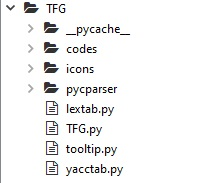
\includegraphics{img/directorios.jpg}
    \caption{Directorios del programa}
    \label{fig:archivos}
\end{figure}

\section{Manual del programador}

Para este apartado se ha optado por un comentario exhaustivo del código en vez mostrar capturas del mismo explicándolo.

\section{Compilación, instalación y ejecución del proyecto}

Para poder usar esta herramienta se deberá tener instalado el paquete de Anaconda 3 para ejecutar el proyecto y MinGW  para compilar los archivos .c que queramos depurar.
Video explicativo de como descargar y ejecutar el proyecto: \url{https://universidaddeburgos-my.sharepoint.com/:v:/g/personal/rmg0094_alu_ubu_es/EV0K9OXoahJDsmgPYIYb6aQB971SI_AAsKBiYx271UNXMg?e=NCeIwd}

\section{Pruebas del sistema}

Pruebas en formato video sobre el funcionamiento de la aplicación

\begin{enumerate}
\item Marca los errores de compilación en rojo: \url{https://universidaddeburgos-my.sharepoint.com/:v:/g/personal/rmg0094_alu_ubu_es/Edqt9ViG2sNHvBCA1C9HLRAB-4638re5Bkyvd5s09D6Wog?e=n0L42k}
\item Los operadores unarios funcionan correctamente: \url{https://universidaddeburgos-my.sharepoint.com/:v:/g/personal/rmg0094_alu_ubu_es/EcdA6aLBDOVFouB1g8PAl9sB7JbkX-I6uyJRMyc-39QNcg?e=vkzMMc}
\item Pruebas de aritmética: \url{https://universidaddeburgos-my.sharepoint.com/:v:/g/personal/rmg0094_alu_ubu_es/EewaAlBQjKJMtqbZ2T4XRDYBErusbBCDNmByTHAcqsOI7Q?e=CFT6gj}
\item Recursividad funciona correctamente: \url{https://universidaddeburgos-my.sharepoint.com/:v:/g/personal/rmg0094_alu_ubu_es/EWCeF2I1IXRDuRUeSp8n8owBw0SxnZ2EAeOna8xsls3Mgw?e=sYuJMS}
\item Llamadas a funciones en cabecera funciona correctamente: \url{https://universidaddeburgos-my.sharepoint.com/:v:/g/personal/rmg0094_alu_ubu_es/ERta1Udad3xHsFfwj98kZQ8B1WsL3LAFof5oyg_MXxXYRQ?e=VO8rGN}
\item Funcionan los scan: \url{https://universidaddeburgos-my.sharepoint.com/:v:/g/personal/rmg0094_alu_ubu_es/EZqjr5tkZO9Eg95EqejMbCkBWbSX5NOXHNXZHnReomZB-A?e=sf5Scb}
\item Los bucles funcionan: \url{https://universidaddeburgos-my.sharepoint.com/:v:/g/personal/rmg0094_alu_ubu_es/Ee5Pp02fZthFrB_YGRNihvUBRQAhyeKK1iu34eACpMqpPg?e=E7B8BX}
\item Los structs se crean correctamente: \url{https://universidaddeburgos-my.sharepoint.com/:v:/g/personal/rmg0094_alu_ubu_es/EdIiHJFhiZJLg9HqHe280xgByZZa6M9pILdKziuY2uVD4g?e=22dJfc}
\item Los arrays se crean correctamente: \url{https://universidaddeburgos-my.sharepoint.com/:v:/g/personal/rmg0094_alu_ubu_es/EfYnYtvseAxFsx3iZl2kS1oBNvREPXqapS9olGLMej1F_A?e=9YdLoK}
\end{enumerate}